\subsection{Coarse grid correction and two grid method}
%\vspace{-1.8cm}
\begin{figure}[hpt]
\begin{center}
\includegraphics*[width=3in]{figures/twogrid.pdf}
%\vspace{-1.5cm}
\caption{Two level grids.} 
\label{Interpolation}
\end{center}
\end{figure} 

\begin{figure}[!htb]
\begin{center}
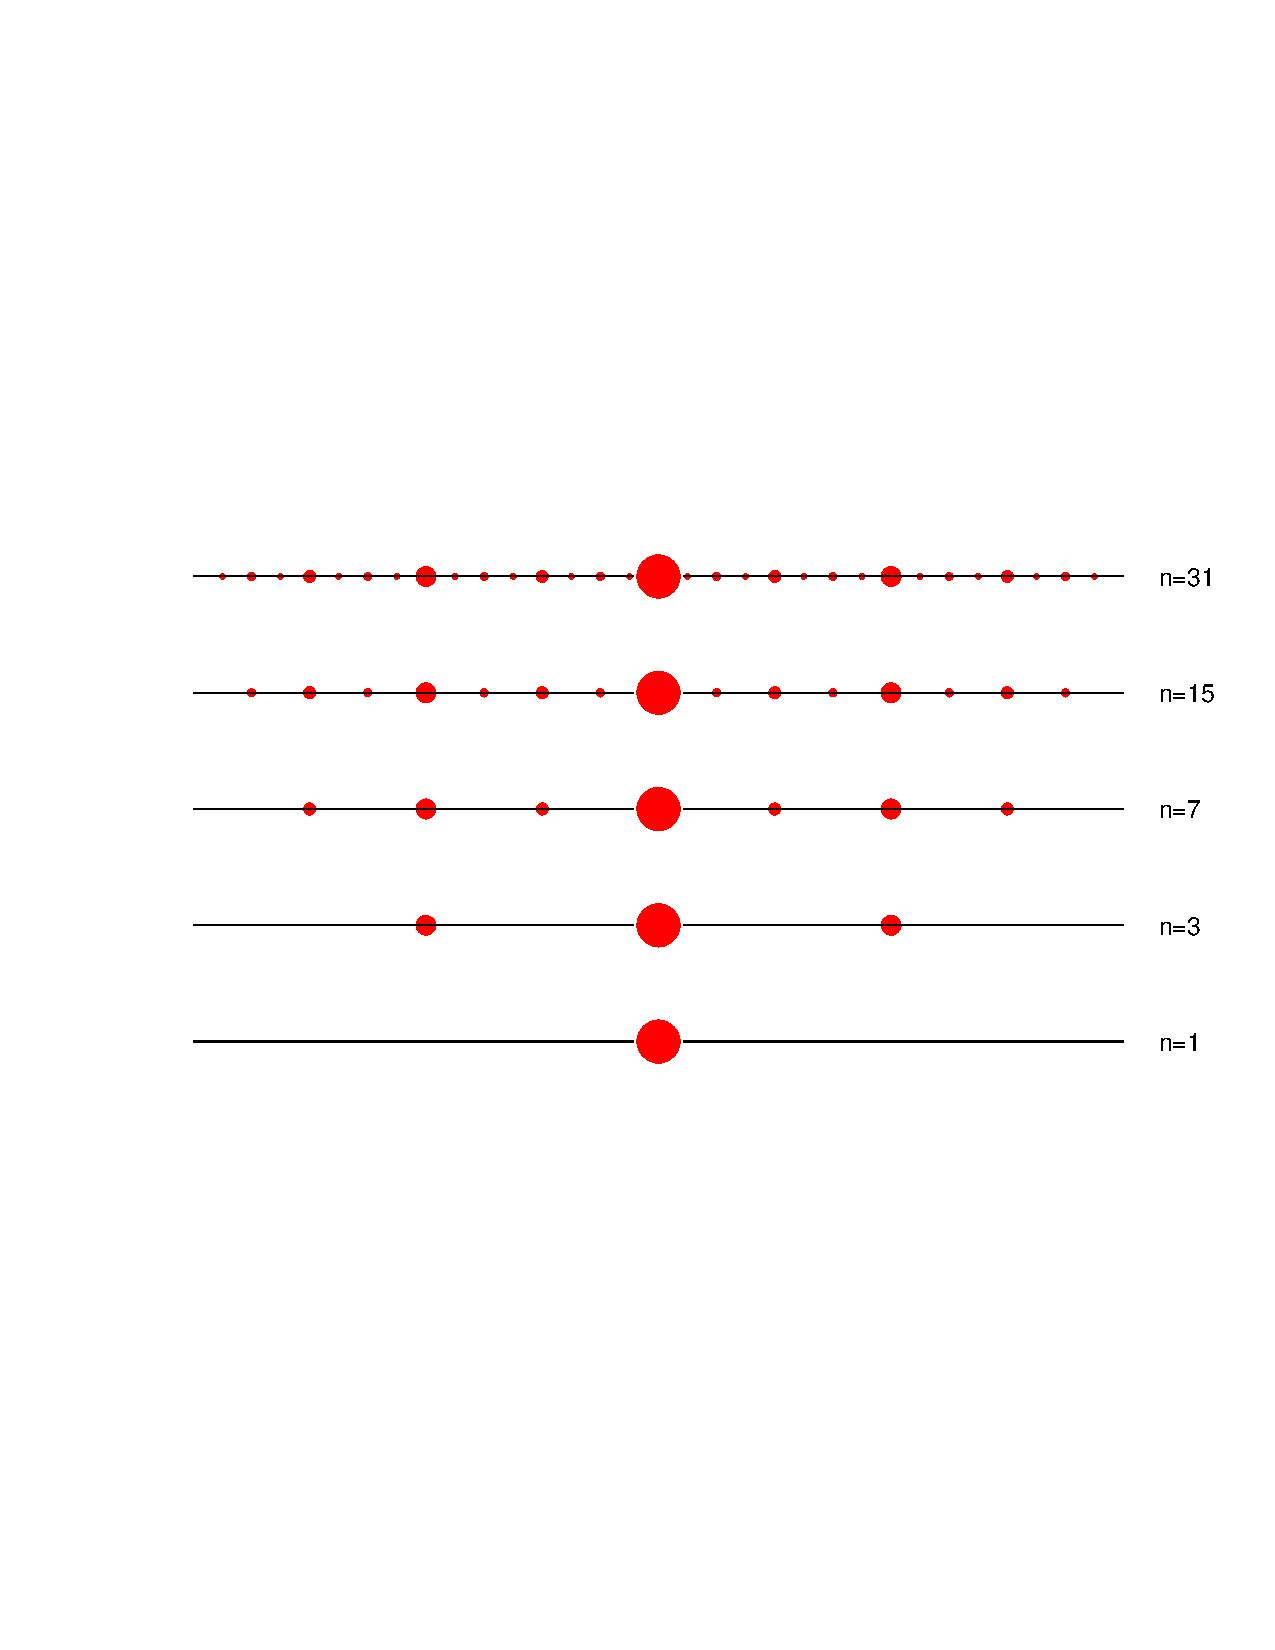
\includegraphics[width=3in]{pictures/manygr.pdf}
\end{center}
\caption{Multiple grids in one dimension
\label{fig:manygrids}}
\end{figure}

%\vspace{-0.2cm}
As we discussed earlier, although gradient descent iteration usually
converges very slowly, it does quickly smooth out the rough 
component in the error. In other words, the error becomes smooth 
after a few gradient descent iterations on a fine grid, but looks 
rough when viewed on a coarser grid. Hence, a few gradient descent
iterations can further reduce the error on the coarse grid. 
The main idea of two grid method or multigrid method is 
to use the fact that a smooth function can be well 
approximated on a coarser grid.  

In summery, we can write the two grid method in terms of finite element (FE) functions as follows:
\begin{algorithm}\caption{A two grid method (in terms of FE functions)}\Label{alg:2grid:opezero}
Input $u^0$.
\begin{enumerate}
\item [{\bf Step 1:}] Apply $\nu_1$-times gradient descent iterations for 
$$
\min_{v^1\in V_1} J(v^1)
$$
with initial guess $u^0$ to obtain $u^1\in V_1$.
\item [{\bf Step 2:}]  Apply $\nu_2$-times gradient descent iterations for 
$$
\min_{v^2\in V_2} J(u^1+v^2)
$$
with zero initial guess to obtain $u^2\in V_2$.
\item [{\bf Step 3:}]  Update: $u=u^1+u^2$.
%\item [{\bf Step 4:}]  Stop if converge or $u^0\update u$ and continue from step 1.
\end{enumerate}
\end{algorithm}
 
\newpage

\subsubsection{Realization of step 1:} 
\smallskip\hrule \smallskip 

Step 1: Given $u^{1,0}\in V_1$, apply $\nu_1$-times gradient descent method for 
$$
\min_{v^1\in V_1} J(v^1)
$$
with initial guess $u^{1,0}$ to obtain $u^1\in V_1$.
\smallskip\hrule \smallskip 


Let $\displaystyle u^{1,0}=\sum_{i=1}^{n_1}\mu^0_i\phi_i^1,\quad v^1=\sum_{i=1}^{n_1}\nu^1_i\phi_i^1,\quad  \mu^0=\{\mu^0_i\}^{n_1}_{i=1},\quad  \nu^1=\{\nu^1_i\}^{n_1}_{i=1}$,

where $\phi^1=(\phi^1_1,\phi^1_2,\cdots,\phi^1_{n_1})$
is the nodal basis of $V_1$. 

Namely, $b^1=b, \mu^1\leftarrow \mu^0$,  for $i=1:\nu_2$ 
$$
\mu^1\leftarrow  \mu^1-\eta_1 (A_1\ast \mu^1-b^1).
$$
After $\nu_1$ iterations, we obtain updated $\mu^1$ and $\displaystyle  u^1=\sum_{i=1}^{n_1}\mu^1_i\phi_i^1$.

\subsubsection{Realization of step 2:} 
\smallskip\hrule \smallskip 
{\bf Step 2:}   Apply $\nu_2$-times gradient descent iterations for 
$$
\min_{v^2\in V_2} J(u^1+v^2)
$$
with zero initial guess to obtain $u^2\in V_2$. 
\smallskip\hrule \smallskip  
Let 
$$
u^1=\sum_{i=1}^{n_1}\mu^1_i\phi_i^1,~v^2=\sum_{i}^{n_2}\nu^2_{i}\phi^{2}_i,~\mu^1=\{\mu^1_i\}^{n_1}_{i=1}, ~ \nu^2=\{\nu^2_{i}\}^{n_2}_{i=1}.$$
We have
\begin{equation}\label{min2h} 
\begin{aligned}
J(u^1+v^2)&=\frac12\int_0^1|(u^1+v^2)'|^2dx-\int_0^1f(u^1+v^2)dx\\
&=J(u^1)+J(v^2)+\int_0^1(u^1)'(v^2)'dx\\
&=\frac12 (\mu^1)^TA_1\ast \mu^1+\frac12 (\nu^2)^TA_2\ast\nu^2-(\nu^2)^Tr^2
\end{aligned}
\end{equation}
where 
\begin{equation}
r_i^2=\int_0^1 f\phi^2_i -(u^1)'(\phi^2_i)'dx=(f,\phi^2_i)-a(u^1,\phi^2_i).
\end{equation}

Now noting that 
\begin{equation}\label{prolongation}
\phi^2_i=\frac12 \phi^1_{2i-1}+ \phi^1_{2i} +\frac12 \phi^1_{2i+1},
\end{equation}
Let $\phi^2=\{\phi^2_i\}_{i=1}^{n_2}, \phi^1=\{\phi^1_i\}_{i=1}^{n_1}$. 
Using the convolution with stride notation,  we obtain 
\begin{equation}\label{rescon}
\phi^2=R\ast_2\phi^1
\end{equation}
with $R=[\frac12,1,\frac12]$.
Furthermore, 
\begin{equation}
\begin{aligned}
r^2_i&=(f, \frac12 \phi^1_{2i-1}+ \phi^1_{2i} +\frac12 \phi^1_{2i+1})-a(u^1,  \frac12 \phi^1_{2i-1}+ \phi^1_{2i} +\frac12 \phi^1_{2i+1})\\
&\displaystyle= \frac12 b^1_{2i-1}+ b^1_{2i} +\frac12 b^1_{2i+1}- \Big(\frac12 (A_1\ast\mu^1)_{2i-1}+   (A_1\ast\mu^1)_{2i}+ \frac12(A_1\ast\mu^1)_{2i+1}\Big)\\
&\displaystyle= \frac12 (b^1-A_1\ast\mu^1)_{2i-1}+ (b^1-A_1\ast\mu^1)_{2i}+\frac12 (b^1-A_1\ast\mu^1)_{2i+1}\\
&\displaystyle= \frac12 r^1_{2i-1}+ r^1_{2i} +\frac12 r^1_{2i+1},
\end{aligned}
\end{equation}
where $r^1=b^1-A_1\ast\mu^1$.
\begin{lemma}
Using the convolution with stride notation, we have $$r^2=R\ast_2r^1$$ with $R=[\frac12,1,\frac12]$.
\end{lemma}
Therefore applying gradient descent method $\nu_2$-times for \eqref{min2h} reads: 

$r^1=b^1-A_1\ast\mu^1, r^2=R\ast_2r^1, \mu^2\leftarrow 0$,
for $i=1:\nu_2 $ 
\begin{equation}
\mu^2\leftarrow \mu^2-\eta_2(A_2\ast \mu^2-r^2). 
\end{equation}
After $\nu_2$ iterations, we obtain updated $\mu^2$ and $\displaystyle  u^2=\sum_{i=1}^{n_2}\mu^2_{i}\phi_i^2$.

\subsubsection{Realization of step 3:} 
\smallskip\hrule \smallskip 
{\bf Step 3:}  $u=u^1+u^2$. 
\smallskip\hrule \smallskip 

Let $\displaystyle  \mu^2=\{\mu^2_{i}\}^{n_2}_{i=1}, \phi^{2}=\{\phi^2_i\}^{n_2}_{i=1}$.
Therefore  $u^2=\sum\limits_{i=1}^{n_2}\mu^2_{i}\phi^2_i
=(\mu^2, \phi^2)_{l^2}$ and by \eqref{rescon} we have
\begin{equation}
\begin{split}
u^2&=(\mu^2, \phi^2)_{l^2}=(\mu^2, R\ast_2\phi^1)_{l^2}=(R\ast_2^{\top}  \mu^2,  \phi^1)_{l^2}\\
&=\sum_{i=1}^{n_1}\left(R\ast_2^{\top} \mu^2\right)_i \phi^1_i
\end{split}
\end{equation}
with $R=[\frac 12,1,\frac12]$.
\begin{lemma}
The prolongation can be written as 
$R\ast_2^T: \mathbb R^{n_2}\rightarrow \mathbb R^{n_1}$, for $\mu^2\in \mathbb R^{n_2}, (R\ast_2^T \mu^2)\in R^{n_1}$ with
$$
(R\ast_2^T \mu^2)_{2i}=\mu^2_i\quad (R\ast_2^T \mu^2)_{2i+1}=\frac 12 (\mu^2_{i+1} +\mu^2_{i}).
$$
\end{lemma}
Noting that $\displaystyle u^1=\sum_{i=1}^{n_1}\mu^1_i\phi_i^1,~\mu^1=\{\mu^1_i\}^{n_1}_{i=1}$, we obtain 
$$
\mu=\mu^1+R\ast_2^T \mu^2\quad\hbox{and}\quad u=u^1+u^2.
$$
%\newpage
Next we show how to realize the Algorithm \ref{alg:2grid:opezero} in vector and convolution form.
%\begin{algorithm}\caption{A two grid method
%$\mu = {\text{2G1}}(b; \mu^0; 2,\nu_1, \nu_2)$}
%\Label{alg:2grid:opecoze}
%Given $\mu^0$.
%\begin{enumerate}
%\item[{\bf Step1:}] 
%
%Set $b^1=b, \mu^1\leftarrow\mu^0$. 
%
%{\bf For} $i=1:\nu_1$ 
%$$
%\mu^1\leftarrow  \mu^1-\eta_1 (A_1\ast \mu^1-b^1).
%$$
%{\bf end for}
%\item [\bf{Step 2:}] Set $r^1=b^1-A_1\ast\mu^1, r^2=R\ast_2r^1,
%  \mu^2\leftarrow 0$. 
%
%{\bf For} $i=1:\nu_2 $ 
%\begin{equation}
%\mu^2\leftarrow \mu^2-\eta_2(A_2\ast \mu^2-r^2). 
%\end{equation}
%{\bf end for}
%\item [{\bf Step 3:}] Update: $\mu=\mu^1+R\ast_2^T \mu^2$.
%\end{enumerate}
%\end{algorithm}

\begin{breakablealgorithm}%[!htb]
	\caption{A two grid algorithm $\mu = {\text{2G1}}(b; \mu^0; 2,\nu_1, \nu_2)$}
\label{alg:L-Slash11d}
\begin{algorithmic}
%	 \State 
%		$$
%		u \leftarrow u^0.
%		$$
	\State Set up
		$$
		b^1 = b, \quad \mu^{1}=\mu^0. 
		$$
		\State Step 1: Smoothing and restriction from fine to coarse level (nested)
		\For{$i = 1:\nu_1$}
		\State
		\begin{equation}\label{eq:smoothing}
		\mu^{1} \leftarrow \mu^{1} + S^1 \ast (b^1 - A_1 \ast \mu^1).
		\end{equation}
		\EndFor
		\State Step 2: Form restricted residual and set initial guess:
		$$
		\mu^{2} \leftarrow 0, \quad b^{2} \leftarrow R \ast_2
                (b^1-  A_1\ast \mu^{1}), 
%A_{2} = R\ast_2 A_1 \ast (R\ast_2^\top).
		$$
		\For{$i = 1:\nu_2$}
		\State
		\begin{equation}\label{eq:smoothing}
		\mu^2 \leftarrow \mu^2+ S^2 \ast (b^2- A_2\ast \mu^2).
		\end{equation}
		\EndFor
		\State Step 3: Prolongation and restriction from coarse to fine level
		\State
		$$
		\mu^{1} \leftarrow \mu^{1} + R  \ast_2^{\top} \mu^{2}.
		$$
		\State
		$$
		\mu \leftarrow \mu^{1}.
		$$
	\end{algorithmic}
\end{breakablealgorithm}





